\documentclass[xetex,mathserif,serif]{beamer}
\usepackage{polyglossia}
\usepackage{minted}
\usepackage{tabu}

\usepackage{textpos}
\setlength{\TPHorizModule}{1cm}
\setlength{\TPVertModule}{1cm}

\useoutertheme{infolines}

\usepackage{fontspec}
\setmainfont{FreeSans}
\newfontfamily{\russianfonttt}{FreeSans}

\definecolor{links}{HTML}{2A1B81}
\hypersetup{colorlinks,linkcolor=,urlcolor=links}

\tabulinesep=0.7mm

\title{Курсовые работы}
\author[Юрий Литвинов]{Yurii Litvinov \newline 
	\textcolor{gray}{\small\texttt{y.litvinov@spbu.ru}}
}

\date{12.02.2018}

\begin{document}
	
	\begin{frame}
		\frametitle{Распознавание жестов мышью в среде визуального моделирования}
		\begin{columns}
			\begin{column}{0.5\textwidth}
				\begin{itemize}
					\item REAL.NET --- среда для создания предметно-ориентированных визуальных языков
					\item \url{https://github.com/yurii-litvinov/REAL.NET}
					\item Рисовать диаграммы неудобно
					\item Рисование диаграмм жестами мыши (или пером)
				\end{itemize}
			\end{column}
			\begin{column}{0.5\textwidth}
				\center{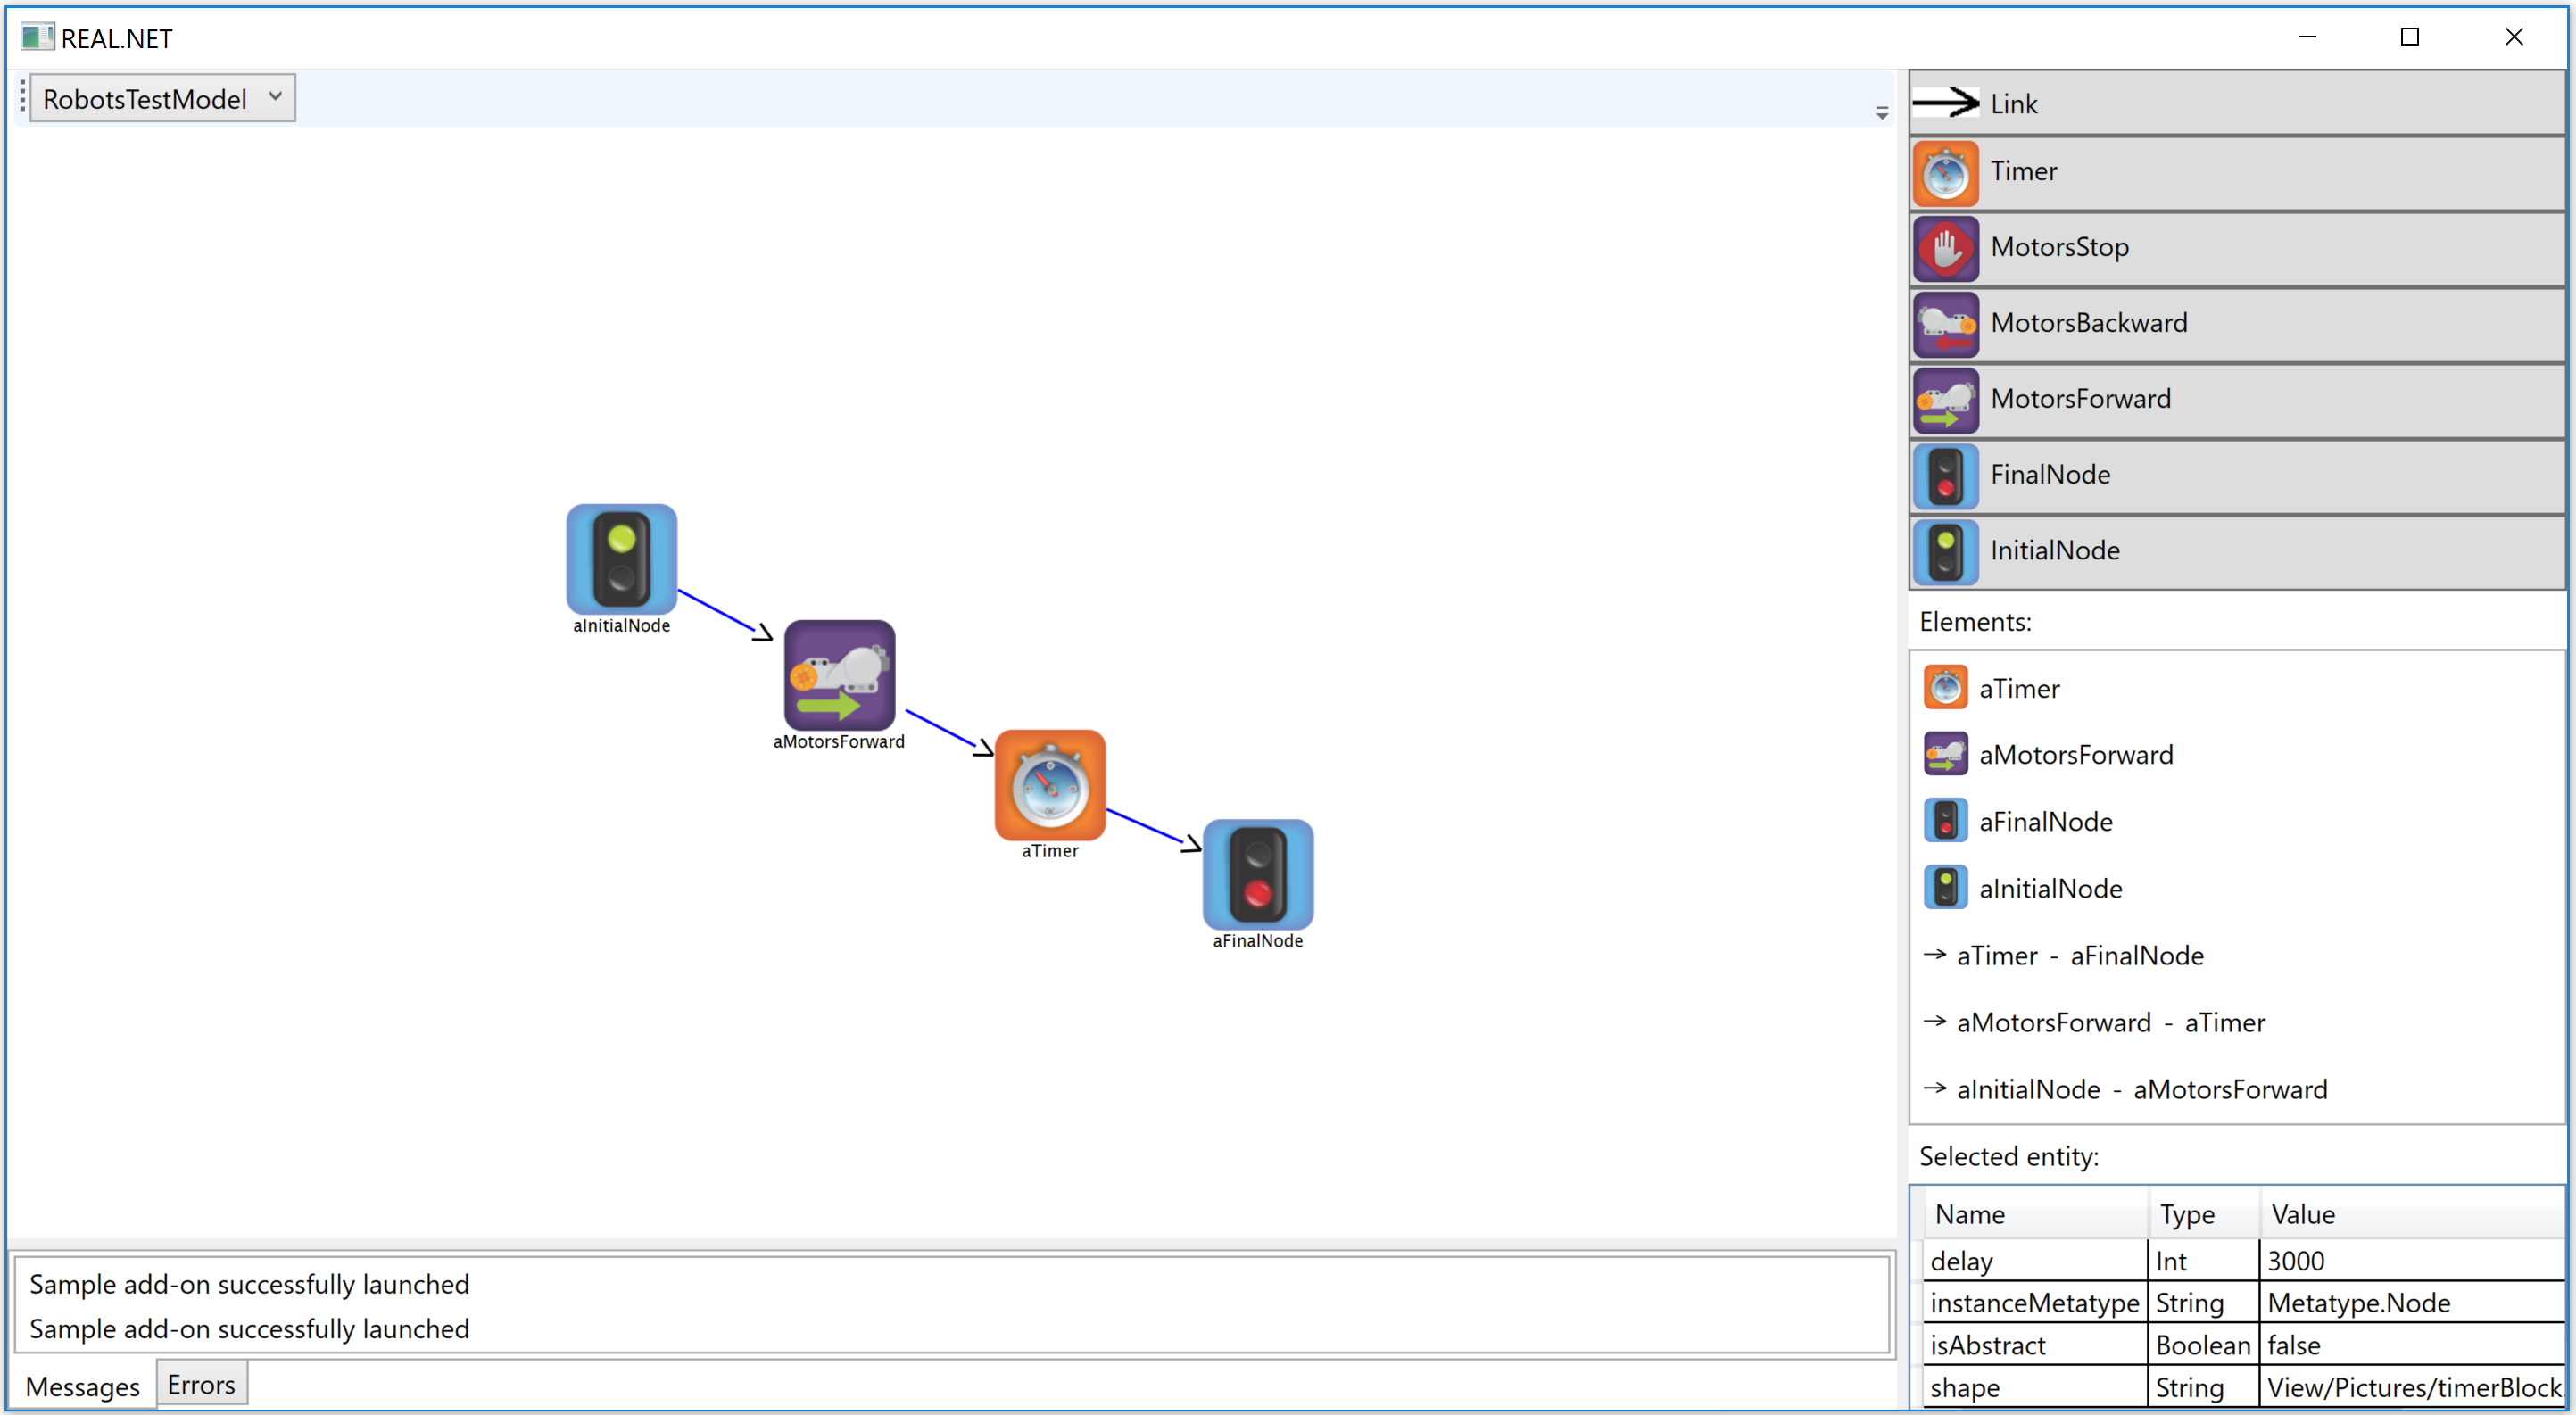
\includegraphics[width=0.98\textwidth]{realNet.png}}

				\center{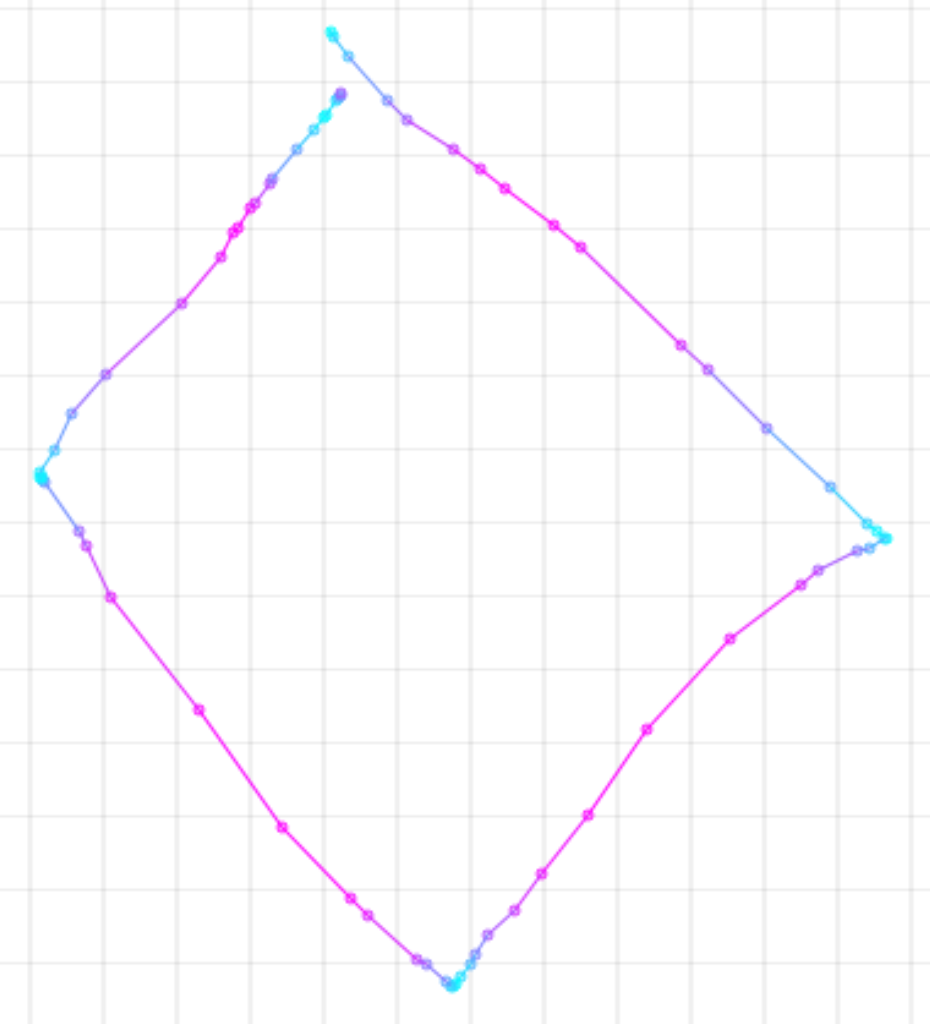
\includegraphics[width=0.3\textwidth]{gesture.png}}
			\end{column}
		\end{columns}
		Технологии: .NET (C\#, F\#), WPF

		Контакты: \texttt{yurii.litvinov@gmail.com}
	\end{frame}

\end{document}

